\section{Document Stores}
\subsection{Einleitung}
Document-Stores speichern strukturierte Daten in Datensätzen, die Dokumente genannt werden. Grundsätzlich vereinigen sie die Schemafreiheit von Key-Value-Stores mit der Möglichkeit zur Strukturierung der gespeicherten Daten. Somit lassen sich Document-Stores als Erweiterung von Key-Value Stores betrachten. Vorteil hierbei ist, dass es bei Document-Stores im Gegensatz zu Key-Value Stores möglich ist komplexere auf den Inhalt (die Attribute) der Dokumente gerichtete Abfragen zu stellen. Dies ist bei Key-Value-Stores nicht möglich.

\subsection{Eigenschaften}
Bei der Betrachtung von Document-Stores bezieht sich das Wort \grqq document\grqq auf die hierarchische Struktur der abgespeicherten Daten. Die hier betrachteten Dokumente bestehen jedoch lediglich aus binären Daten oder einfachem Text. Ferner kann es sich um Semi-strukturierte Daten wie JSON oder XML handeln. Während ältere Document-Stores auf XML setzten, ist bei neueren Document-Stores das JSON ähnliche BSON üblich. 
\\

In einer Document-Store basierten NoSQL-Datenbank ist es möglich beliebigen Daten zu speichern, ohne das die Datenbank im Vorfeld Wissen über die Struktur der Daten hat oder weiß was die Daten bedeuten. Gegenüber relationalen Datenbanken bietet dies den Vorteil, dass das Datenbankschema bei kleinen Änderungen nicht großartig verändert werden muss \cite{harrison01}. 
\\

In einer Document-Store Datenbank ist folgende Hierarchie typischerweise anzutreffen:
\begin{itemize}
\item Ein Dokument ist eine Grundeinheit für das speichern von Daten. Sie ist zu vergleichen mit einer Zeile einer Relationalen Datenbank.
\item Ein Dokument besteht aus einem oder mehreren Key-Value Paaren, und kann weitere Dokumente und Arrays enthalten. die Arrays können wiederum ebenfalls Dokumente enthalten, was eine komplexere Strukturierung ermöglicht.
\item eine Sammlung oder ein Data Bucket ist ein Set von Dokumenten, die einen Zweck teilen. Dies ist äquivalent zu einer relationalen Tabelle. Hier ist jedoch relevant zu erwähnen, dass die Dokumente hier nicht vom gleichen Typ sein müssen, auch wenn es üblich ist, dass solche Dokumente die gleiche Art von Information darstellen \cite{harrison01}.
\end{itemize}

\subsection{Datenmodell}
Im Zentrum des Datenmodells der Document-Stores stehen die Documents, die eine hierarchische Struktur aufweisen. So kann ein Dokument auf viele weitere Dokumente verweisen. Dies ist möglich, da ein Dokument Listen enthalten kann. 
\\

Wie bereits erwähnt ist es möglich mithilfe von Document-Stores ein relationales Schema nachzubilden. Dies ist jedoch häufig nicht sinnvoll, da es größere Vorteile bringt die Dokumente in kleineren Sammlungen zusammenzufassen und in eingebetteten Dokumente die größte Detailstufe zu bieten \cite{harrison01}. 
\\

Sei \ref{fig:doc2} die Darstellung einer relationalen Datenbank mit Filmen und Schauspielern.
\begin{figure}[H]
	\centering
	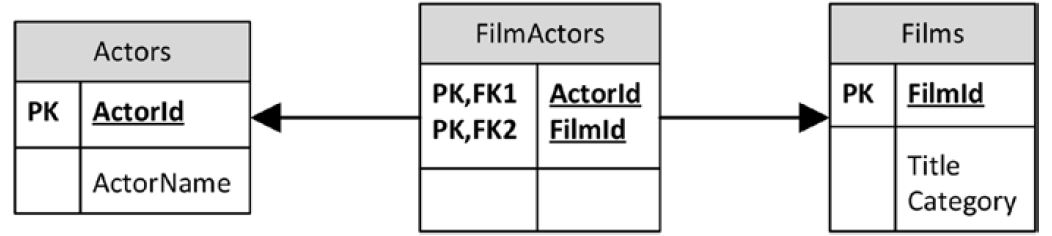
\includegraphics[scale=0.4]{images/docstores_2.jpg} 
	\caption{Beispiel eines JSON-Dokuments}\label{fig:doc2}
\end{figure}
In einer relationalen Datenbank würde es eine Tabelle mit Filmen und eine Tabelle mit Schauspielern geben, die zu einer gemeinsamen Tabelle gejoint werden würden um anzuzueigen welcher Schauspieler bei welchem Film mitgewirkt hat. Mithilfe von Document-Stores wäre dieses Schema so auch möglich, jedoch gibt es hierfür einen besseren Ansatz. Da Document-Stores grundsätzlich keine Join-Operationen ermöglichen und Entwickler es bevorzugen wenn die JSON Strukturen sich nah an dem objektorientierten Programmentwurf orientieren, bietet sich ein Entwurf nach \ref{fig:doc1} eher an \cite{harrison01}.
\begin{figure}[H]
	\centering
	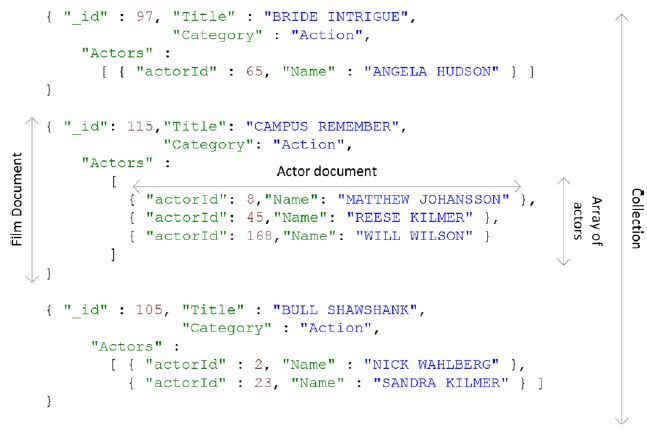
\includegraphics[scale=0.75]{images/docstores_1.jpg}
	\caption{Beispiel eines JSON-Dokuments}\label{fig:doc1}
\end{figure}
Wie in der Abbildung \ref{fig:doc1} zu sehen, befindet sich ein Array von Schauspieler Dokumenten in dem Film Dokument. Dieser Design-Entwurf, der Document-Embedding genannt wird, hat den Vorteil, dass hierdurch auf aufwendige Join-Operationen verzichtet werden kann. Nachteil hierbei ist jedoch, dass die Schauspieler in vielen Dokumenten auftauchen und somit redundant sind. Sollte zudem eines der Schauspieler Attribute verändert werden müssen kann dies zu Inkonsistenzen führen. Ein weiteres Problem kann auftreten, wenn beispielsweise eine unbegrenzte Anzahl an Schauspielern möglich sein soll, da Dokumente in der Regel begrenzt sind. Um dieses Problem zu lösen besteht jedoch die Möglichkeit Indizes zu verwenden \cite{harrison01}.
\begin{figure}[H]
	\centering
	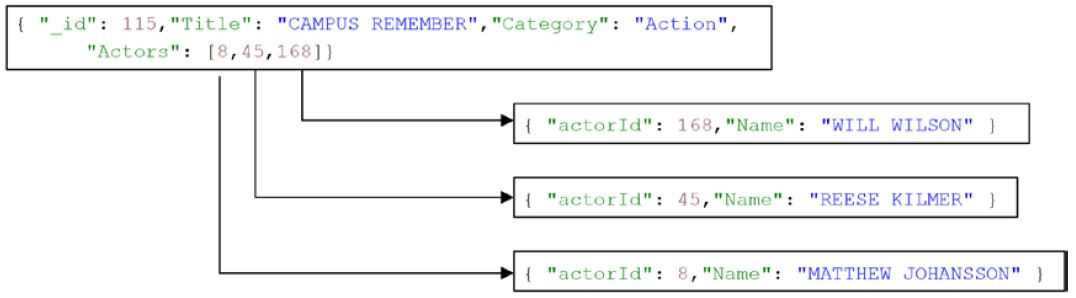
\includegraphics[scale=0.5]{images/docstores_3.jpg} 
	\caption{Beispiel eines JSON-Dokuments}\label{fig:doc3}
\end{figure}
In Abbildung \ref{fig:doc3} ist zu sehen, wie ein solches System aussehen könnte. 
\\

Grundsätzlich gilt bei modernen Document-Stores, dass Dokumente üblicherweise in JSON bzw. BSON vorliegen \cite{harrison01}.

\subsubsection{JSON}
Die Java-Script-Object-Notation ist ein vom Menschen und Maschinen lesbarer Standard zur Beschreibung von Daten. JSON ist wie XML ein Standard zum Datenaustausch im Web.
In \ref{fig:doc1} ist ein Beispiel für ein JSON-Dokument zu sehen. Vorteil von JSON ist, dass JSON-Dokumente einfach zu zerlegen und umzuwandeln sind. Dies verringert den Aufwand, der in der Anwendungsschicht betrieben werden muss.
\subsubsection{BSON}
Unter BSON sind binär kodierte JSON-Dokumente zu verstehen. BSON erweitert das Modell von JSON um weitere Datentypen und ermöglicht effizientes kodieren und dekodieren innerhalb verschiedener Sprachen.
\subsection{Anwendungsfälle}
JSON basierte Document-Stores haben vor allem in Web-basierten Anwendungen ihre Vorzüge. Hier wird häufig JSON als Datenschicht verwendet, weswegen Document-Stores hier bevorzugt werden.
\\

XML-basierte Document-Stores finden vor allem in Content-Management-Systemen Anwendung, da sie hier ein Management Repository für XML-basierte Textdateien zur Verfügung stellen.
\\

Grundsätzlich lässt sich jedoch feststellen:
\begin{itemize}
\item dass Document-Stores vor allem in Umgebungen florieren, in denen über viele Wege Zugang zu den Daten gewährleistet werden soll, die wiederum vielfältiger Natur sein können. 
\item dass Document-Stores sinnvoll sind, wenn eine große Menge an kleinen, sich wiederholenden Schreib- und Lesevorgängen abgearbeitet werden muss.
\item dass Document-Stores sinnvoll sind, wenn die CRUD-Operationen ohne großartige Join-Operationen umgesetzt werden sollen.
\item dass Document-Stores sinnvoll sind, wenn eine programmiererfreundliche Datenbank umgesetzt werden soll.
\end{itemize}

\subsection{Bewertung}
Hieraus lässt sich evaluieren, dass Document-Stores vielfältige Einsatzmöglichkeiten haben. Vor allem im Bereich der Web-Technologien haben Document-Stores wie MongoDB Stärken, die sie zu guten Alternativen zu klassischen relationalen Datenbanken machen. Durch die Freiheiten bei den zu speichernden Daten und der Einfachheit der Abfragen zeigen sich hier vor allem ihre Stärken. Ferner wird deutlich, dass, gemessen an der Geschwindigkeit in der neue Technologien zur Darstellung von Daten entstehen, Document-Stores im Web die notwendige Freiheit bieten, um angemessen vorzugehen.